\documentclass[11pt,letterpaper,boxed]{hmcpset}
\usepackage{fullpage}
\setlength{\parskip}{6pt}
\setlength{\parindent}{0pt}
\usepackage[margin=1in]{geometry}
\usepackage{graphicx}
\usepackage{enumerate}
\usepackage{marvosym}
\usepackage{amssymb}
\usepackage{wasysym}
\usepackage{gensymb}
\usepackage{mathrsfs}
\usepackage{scrextend}
\usepackage{mathtools}
\usepackage{pgfplots}
\usepackage{xspace}

\name{Box \#$\rule{1cm}{0.15mm}$}
\class{Physic 51 Section $\rule{.5cm}{0.15mm}$}
\assignment{Problem Set 2}
\duedate{17 September 2018}

\begin{document}

%\begin{center}
\noindent\textbf{Collaborators:} 
%\end{center} 

%\problemlist{}

\begin{problem}[HRK P27.3 \textbf{Solo}]
A small sphere whose mass $m$ is $1.12$ mg carries a charge $q = 19.7$ nC. It hangs in the in the Earths gravitational field from a silk thread that makes an angle $\theta = 27.4^{\deg}$ with a large, uniformly charged, non conducting sheet as in Fig. 27-32. Calculate the uniform charge density $\sigma$ for the sheet
\begin{center}
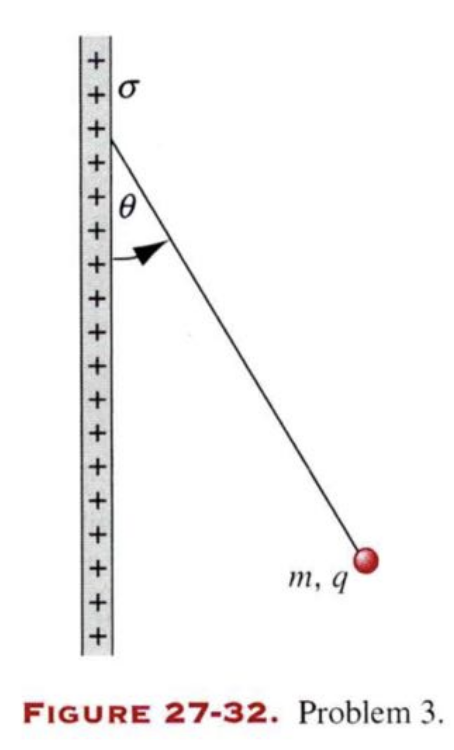
\includegraphics[scale=0.6]{27-32.png}
\end{center} 
\end{problem}

\begin{solution}
\vfill
\end{solution}
\newpage

\begin{problem}[HRK P27.7]
A point charge $+q$ is a distance $d/2$ from a square surface of side $d$ and is directly above the center of the square as shown in Fig. 27-26. Find the electric flux through the square. (Hint: Think of the square as one face of a cube with edge $d$ 
\begin{center}
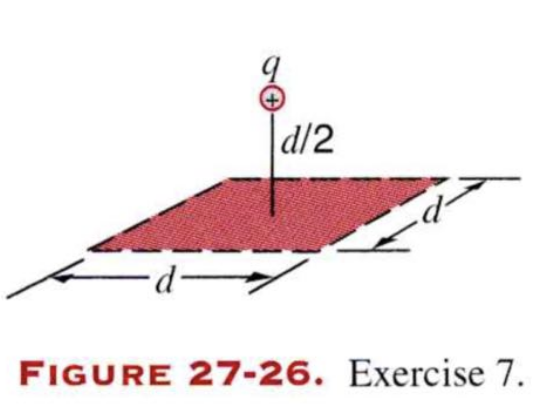
\includegraphics[scale=0.6]{27-26.png}
\end{center} 

\end{problem}

\begin{solution}
\vfill
\end{solution}
\newpage

\begin{problem}[HRK P27.16	]
A plane slab of thickness $d$ has a uniform volume charge density of $\rho$. Find the magnitude of the electric field at all points in space both $(a)$ inside and $(b)$ outside the slab in terms of $x$ the distance measured from the median plane of the slab. 
\end{problem}

\begin{solution}
\vfill
\end{solution}
\newpage

\begin{problem}[HRK P27.17]
A solid nonconducting sphere of radius $R$ carries a nonuniform charge distribution, with charge density, $\rho= \rho_Sr/R$, where $\rho_S$ is a constant and $r$ is the distance from the center of the sphere. Show that $(a)$ the total charge on the sphere  is $Q= \pi \rho_sR^3$ and $(b)$ the electric field inside the sphere is given by; 
$$ E = \frac{1}{4\pi \epsilon_0}\frac{Q}{R^4}r^2$$
\end{problem}

\begin{solution}
\vfill
\end{solution}
\newpage

\begin{problem}[HRK P27.4]
Figure 27-33 shows a charge $+q$ arranged as a uniform conducting sphere of radius $a$ and placed at the center of a spherical conducting shell of inner radius $b$ and outer radius $c$. The outer shell carries a charge of $-q$. Find $E(r)$ at locations $(a)$ within the sphere, $(r<a), (b)$ between the sphere and the shell, $(a<r<b). (c)$ Inside the shell $(b<r<c )$ and $(d)$ outside the shell $(r>c). (e)$ What charges appear on the inner and outer surfaces of the shell. 
\begin{center}
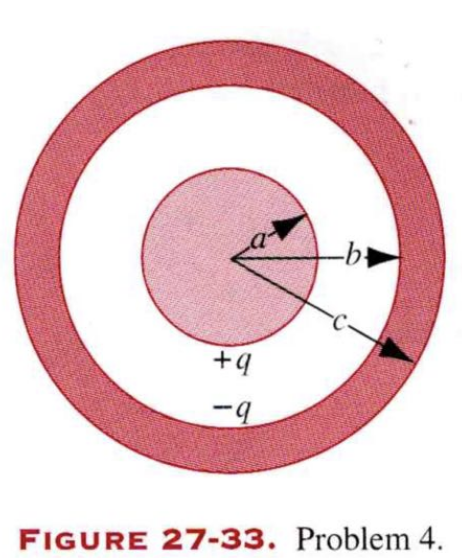
\includegraphics[scale=0.6]{27-33.png}
\end{center}
\end{problem}

\begin{solution}
\vfill
\end{solution}
\newpage

\begin{problem}[HRK E29.29]
A $1-\mu C$ point charge is embedded in the center of  a solid pyrex sphere of radius $R=10$cm. $(a)$ Calculate the electric field strength $E$ just beneath the surface of the sphere. $(b)$ Assuming that there are no other \textit{free} charges, calculate the strength of the electric field just outside the surface of the sphere. $(c)$ What is the induced surface charge density $\sigma_{ind}$ on the surface of the Pyrex sphere? 
\end{problem}

\begin{solution}
\vfill
\end{solution}

\end{document}